\documentclass[11pt]{article}
\usepackage[margin=1in, top=1in]{geometry}
\usepackage[all]{nowidow}
\usepackage[hyperfigures=true, hidelinks, pdfhighlight=/N]{hyperref}
\usepackage[separate-uncertainty=true, group-digits=false]{siunitx}
\usepackage{graphicx,amsmath,physics,tabto,float,amssymb,pgfplots,verbatim,tcolorbox}
\usepackage{listings,xcolor,subcaption,caption,import,wrapfig,minted}
\usepackage[sorting=none]{biblatex}
\usepackage[version=4]{mhchem}
\usepackage[noabbrev]{cleveref}
\usepackage[british]{babel}
\newcommand{\creflastconjunction}{, and\nobreakspace}
\newcommand{\mb}[1]{\mathbf{#1}}
\numberwithin{equation}{section}
\numberwithin{figure}{section}
\numberwithin{table}{section}
\captionsetup{font=small, belowskip=0pt}
\pgfplotsset{compat=1.17}
\addbibresource{bibliography.bib}
\usemintedstyle{vs}
\definecolor{LightGray}{HTML}{eaeaea}
\setminted{framesep=2mm,bgcolor=LightGray,fontsize=\footnotesize,linenos,breaklines}
\let\OldTexttt\texttt
% \sethlcolor{LightGray}
\renewcommand{\texttt}[1]{\OldTexttt{\hl{#1}}}

\begin{document}

\begin{center}
    {\huge 1032F Test 1a Solutions}\\
    \vspace{0.2in}
    
    
\end{center}

\section*{Questions}

\begin{enumerate}
    \item \begin{enumerate}
        \item What is the potential difference between two points that are situated \SI{10}{\centi\metre} and \SI{20}{\centi\metre} from a \SI{3.0}{\micro\coulomb} charge?
        \item To what location should the point at \SI{20}{\centi\metre} be moved to double that potential difference?
    \end{enumerate}

    \item \begin{enumerate}
        \item Find the current through each of these four resistors.
        \item Find the voltage across each of these four resistors.
        
        \begin{figure}[h]
            \begin{center}
                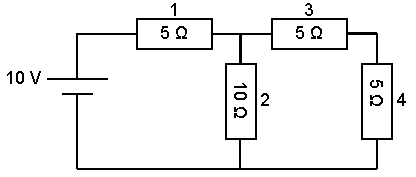
\includegraphics[width=.8\textwidth]{circuit.pdf}
            \end{center}
        \end{figure}
        
    \end{enumerate}

    \item An electron is accelerated from rest by a potential difference of \SI{350}{\volt}. It then enters a uniform magnetic field of magnitude \SI{200}{\milli\tesla} with its velocity perpendicular to the field. Calculate
    \begin{enumerate}
        \item the speed of the electron.
        \item the radius of its path in the magnetic field.
    \end{enumerate}
\end{enumerate}

\section*{Answers}

\begin{enumerate}
    \item \begin{enumerate}
        \item The potential due to a point charge $q$ at a distance $r$ away from that point charge is given by $V=\frac{1}{4\pi\epsilon_0}\frac{q}{r}$. So
        
        \begin{align*}
            V_1 &= \SI{9e9}{\kilo\gram\cdot\metre\cubed\second^{-4}\ampere^{-2}}\frac{\SI{3e-6}{\coulomb}}{\SI{0.01}{\metre}} = \SI{2.7e5}{\volt}\\
            V_2 &= \SI{9e9}{\kilo\gram\cdot\metre\cubed\second^{-4}\ampere^{-2}}\frac{\SI{3e-6}{\coulomb}}{\SI{0.02}{\metre}} = \SI{1.35e5}{\volt}
        \end{align*}

        We can find the potential difference by subtracting one from the other. For convenience we subtract the smaller from the larger.

        \begin{equation*}
            \Delta V = V_1-V_2 = \underline{\SI{1.35e5}{\volt}}
        \end{equation*}

        \item In order to double the potential difference, we require
        
        \begin{align*}
            \Delta V &= \SI{2.7e5}{\volt} \\
            \implies \SI{2.7e5}{\volt} &= \SI{2.7e5}{\volt} - V_2 \\
            \implies V_2 &= 0
        \end{align*}

        In order for the potential at a point to be zero, we must have that point be infinitely far from the charge. Thus the point must be \underline{moved to infinity} in order to double the potential difference.
    \end{enumerate}

    \item \begin{enumerate}
        \item To find the current through the whole circuit we first need to find the resistance of the whole circuit. $R_3$ and $R_4$ just add as they are in series, then that must be combined with $R_2$ according to the parallel rules, then finally we can add that to $R_1$ as it is in series.
        
        \begin{align*}
            R_{tot} &= R_1 + \frac{1}{\frac{1}{R_2} + \frac{1}{R_3 + R_4}} \\
            &= \SI{5}{\ohm} + \frac{1}{\frac{1}{\SI{10}{\ohm}} + \frac{1}{\SI{5}{\ohm} + \SI{5}{\ohm}}} \\
            &= \SI{10}{\ohm}
        \end{align*}

        Then the total current is simply $I = \frac{V}{R_{tot}} = \SI{1}{\ampere}$. 
        
        The current through elements in series is all identical so \underline{$I_1=\SI{1}{\ampere}$}. Then since $R_2=R_3+R_4$, the current splits equally between $R_2$ and the $R_{3,4}$. Thus \underline{$I_2=\SI{0.5}{\ampere}$} and \underline{$I_{3,4}=\SI{0.5}{\ampere}$}.

        \item Finding the voltage across each resistor is now simple as we know the current and the resistance, so we just use $V=IR$.
        
        \begin{equation*}
            \underline{V_1 = \SI{5}{\volt},\;\;\;V_2 = \SI{5}{\volt},\;\;\;V_3 = \SI{2.5}{\volt},\;\;\;V_1 = \SI{2.5}{\volt}}
        \end{equation*}
    \end{enumerate}

    \item \begin{enumerate}
        \item From the definition of an electron volt, an electron gains \SI{1}{\electronvolt} of energy when accelerated by one Volt of potential difference. So the electron gains \SI{350}{\electronvolt}. Converting this to Joules we find \SI{5.6e-17}{\joule}. This is its kinetic energy, so we can find the velocity from $E_K = \frac{1}{2}m v^2$:
        
        \begin{align*}
            v &= \sqrt{\frac{2E_K}{m}} \\
            &= \sqrt{\frac{2\cdot \SI{5.6e-17}{\joule}}{\SI{9.1e-31}{\kilo\gram}}} \\
            &= \underline{\SI{11.09e6}{\metre\second^{-2}}}
        \end{align*}

        \item The radius of its path is simply found from $r = \frac{mv}{qB}$. We can simply plug the values in and find
        
        \begin{equation}
            r=\frac{\SI{9.1e-31}{\kilo\gram}\cdot \SI{11.09e6}{\metre\second^{-2}}}{\SI{1.6e-19}{\coulomb}\cdot\SI{200e-3}{\tesla}}=\underline{\SI{3.155e-4}{\metre}}.
        \end{equation}
        
    \end{enumerate}
\end{enumerate}

\end{document}